\subsubsection{Data Operations}
\label{sec:data_operations}

Two RMB context menus exist in the 'Layers' tab: the layer-tree menu (Data Operations) and the items-panel menu (Item Operations). Both share a set of Common Operations described at the end of this section. \\

\paragraph{Data Operations}
\begin{figure}[H]
    \centering
    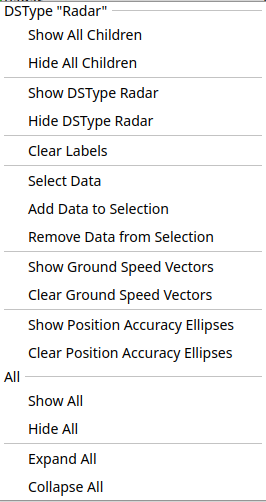
\includegraphics[width=5.5cm,frame]{figures/geoview_layer_context_menu.png}
  \caption{Geographic View layer context menu}
\end{figure}

Opened by a RMB click on an entry in the layer tree. The header line shows the clicked scope: 'DSType "<name>"', 'Data Source "<name>"', 'Line "<name>"', or 'DBContent "<name>"'. Menu-specific entries:

\begin{itemize}
 \item Show All Children / Hide All Children: Show or hide every direct child (group items only)
 \item Show <scope> / Hide <scope>: Show or hide this node (e.g. 'Show DSType Radar')
\end{itemize}

A tree-wide 'All' section is appended at the bottom of every layer context menu:

\begin{itemize}
 \item Show All / Hide All: Show or hide every entry in the tree
 \item Expand All / Collapse All: Expand or collapse every row
\end{itemize}

\paragraph{Item Operations}
\begin{figure}[H]
    \centering
    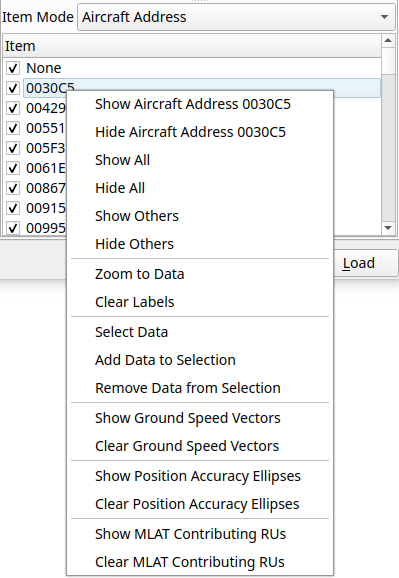
\includegraphics[width=9cm,frame]{figures/geoview_item_context_menu.png}
  \caption{Geographic View item context menu}
\end{figure}

Opened by a RMB click on an entry in the items panel (the list below the layer tree, grouped by the current 'Item Mode'). Menu-specific entries:

\begin{itemize}
 \item Show <grouping> <item> / Hide <grouping> <item>: Show or hide the clicked item (e.g. 'Show Aircraft Address 0030C5'). Only shown when the click hits an item row.
 \item Show All / Hide All: Show or hide every item in the panel
 \item Show Others / Hide Others: Show or hide all sibling items. Only shown when the click hits an item row and at least 2 items exist.
 \item Zoom to Data: Center the map on the clicked item's data extent
\end{itemize}

\paragraph{Common Operations}

The following entries appear in both the Data Operations and Item Operations menus, applied to the clicked scope or item:

\begin{itemize}
 \item Clear Labels: Remove all labels in scope
 \item Select Data: Select (only) target reports in scope
 \item Add Data to Selection: Add target reports in scope to the selection
 \item Remove Data from Selection: Remove target reports in scope from the selection
 \item Show Ground Speed Vectors / Clear Ground Speed Vectors
 \item Show Position Accuracy Ellipses / Clear Position Accuracy Ellipses
\end{itemize}

Conditional entries:

\begin{itemize}
 \item Show / Clear ARTAS Target Report Usage: Only if ARTAS Target Report Usage information was calculated and the scope contains system track updates.
 \item Show / Clear Ground Lines: Only if 'Use Height' is active. Shows / clears connection lines to the ground for all target reports in scope.
 \item Show / Clear MLAT Contributing RUs: Only if MLAT Remote Unit information is present (see \nameref{sec:ui_configure_ds_mlat_rus}). Shows / clears connection lines between target reports and the contributing MLAT Remote Units.
\end{itemize}
